\subsection{Captura e identificação de imagem}

A tecnologia vem crescendo cada vez mais em todo mundo, proporcionando a ampliação do uso de dispositivos de alto desempenho. Paralelo a isso, o fluxo de dados aumenta proporcionalmente, exigindo uma velocidade de conexão maior com a Internet. Um exemplo disso são os \textit{smartphones}, que se popularizaram por serem dispositivos multifuncionais, podendo ser utilizados para tarefas profissionais e pessoais. 

Por conseguinte deste avanço científico, é notório a grande evolução na utilização de imagens digitais em várias áreas, como, por exemplo, em transmissões de TV, conteúdos via \textit{streaming}, imagens capturadas por satélite e até mesmo imagens transmitidas pelas redes sociais. No entanto, como funciona a captura de uma imagem em tempo real? Qual o conceito de imagem?

Uma imagem digital pode ser considerada como sendo uma matriz de pontos elementares, em que cada ponto recebe o nome de \textit{pixel}. Quanto maior a quantidade de \textit{pixels} melhor a resolução da imagem e consequentemente maior o seu tamanho. Cada \textit{pixel} é representado por um valor que indica a intensidade de brilho, denominado nível de cinza, e a quantidade de níveis de cinza depende da quantidade de bits usada na representação de cada \textit{pixel} \cite{SOUZA2007}.

Sendo assim, a matriz de pontos elementares de uma imagem digital pode ser representada conforme na \autoref{fig_imagem-digital-monocromatica}.

\begin{figure}[h]
	\caption{\label{fig_imagem-digital-monocromatica}Representação de uma imagem digital ampliada ao limite dos pixels.}
	\begin{center}
		\resizebox{.3\linewidth}{!}{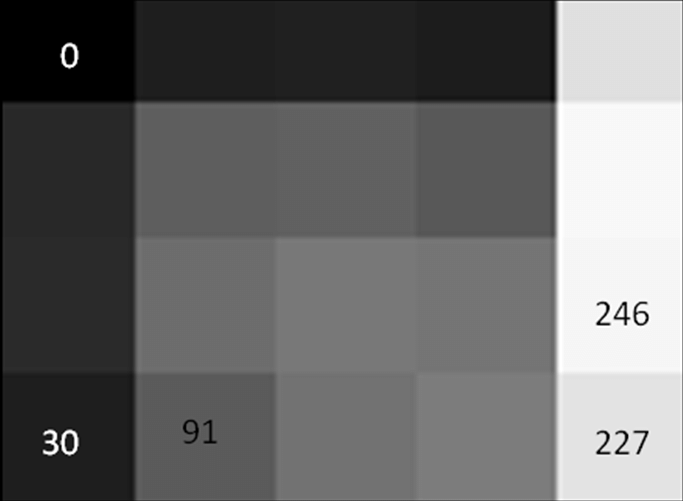
\includegraphics{4-Conteudo-Bibliografico/2-Visao-Computacional/Imagens-Visao-Computacional/representacao-img-digital.png}}
	\end{center}
	\centering \legend{Fonte: \citeonline{STANOJEV2017}}
\end{figure}

A captura e identificação em tempo real de uma imagem consiste em analisar um ambiente tridimensional e elaborar digitalmente uma imagem 2-D (duas dimensões), ocasionando uma imagem estática daquele ambiente tridimensional selecionado. Esse conceito está relacionado a perspectiva, segundo \citeonline{PERONTI2008}. Para que isso seja possível, é necessário utilizar um dispositivo capaz de realizar essa ação, ou seja, uma câmera digital, \textit{smartphones}, dentre outros.

Segundo \citeonline{CHMIELEWSKI2009}, isso se tornou capaz devido a uma tecnologia que surgiu nos anos 70 denominada CCD, \textit{Charge Coupled Device} (dispositivo acoplado de carga): “O sensor CCD ou dispositivo de carga acoplada é uma matriz de elementos sensíveis à luz, fabricados utilizando tecnologia MOS, \textit{Metal Oxide Semiconductor} (semicondutor de óxido metálico), onde cada \textit{pixel} pode ser considerado como um capacitor MOS.”

Atualmente, o sensor mais utilizado nos dispositivos de captura de imagem são de sistemas digitais CMOS - \textit{Complementary Metal Oxide Semiconductor} (semicondutor complementar de óxido metálico), que surgiu nos anos 90 devido a um protótipo do sensor de imagem APS - \textit{Active Pixel Sensor} (Sensor de pixel ativo) criado pela NASA - \textit{National Aeronautics and Space Administration} (Administração Nacional Aeronáutica e Espacial), que possibilitou a fabricação direta de funções como \textit{zoom}, diferentes resoluções de aquisições, acesso aleatório, etc., podendo executar todas as funções do CCD. “Os sensores de imagem APS são formados por elementos sensíveis à luz, capazes de gerar um sinal elétrico ou carga proporcional à intensidade da luz que incide sobre eles.” \cite{CHMIELEWSKI2009}